\documentclass[letterpaper,twocolumn,10pt]{article}
\usepackage{deps/usenix-2020-09}

% The preceding line is only needed to identify funding in the first footnote.
% If that is unneeded, please comment it out.
\usepackage{cite}
\usepackage{amsmath,amssymb,amsfonts}
\usepackage{algorithmic}
\usepackage{graphicx}
\usepackage{textcomp}
\usepackage{xcolor}
\def\BibTeX{{\rm B\kern-.05em{\sc i\kern-.025em b}\kern-.08em
    T\kern-.1667em\lower.7ex\hbox{E}\kern-.125emX}}

%-------------------------------------------------------------------------------
% INCLUDES
%-------------------------------------------------------------------------------

\usepackage{acronym}
\usepackage{xspace}
\usepackage{xstring}
\usepackage{tikz}
\usepackage{hyperref}
\usepackage{censor}
\usepackage{multirow}
\usepackage{booktabs}
\usepackage{makecell}
\usepackage{listings}
\usepackage{relsize}
\usepackage{xcolor}
\usepackage{nimbusmono}
\usepackage[T1]{fontenc}
\usepackage{underscore}
\usepackage{tcolorbox}
\usepackage{enumitem}
\usepackage[explicit]{titlesec}
\usepackage{subcaption}
\usepackage{lipsum}
\usepackage{tabularx}
\usepackage{graphicx}
\usepackage{siunitx}
\usetikzlibrary{arrows.meta}
    % all additional packages.
% !TEX root = main.tex
% Author Macros
\newcounter{gm} % Gwangmu 
\newcounter{du} % Duo 
\newcounter{so} % Solmaz 
\newcounter{by} % Byoungyoung
\newcounter{ma} % Mathias

%\def\enablecomm{1}  % NOTE: comment this out to disable comments.
\ifx\enablecomm\undefined
  \newcommand{\gm}[1]{}
  \newcommand{\du}[1]{}
  \newcommand{\so}[1]{}
  \newcommand{\by}[1]{}
  \newcommand{\mat}[1]{}
\else
  \newcommand{\gm}[1]{\textcolor{teal}{\{Gwangmu-\arabic{gm}: #1\}}\addtocounter{gm}{1}}
  \newcommand{\du}[1]{\textcolor{red}{\{Duo-\arabic{du}: #1\}}\addtocounter{du}{1}}
  \newcommand{\so}[1]{\textcolor{orange}{\{Solmaz-\arabic{so}: #1\}}\addtocounter{so}{1}}
  \newcommand{\by}[1]{\textcolor{blue}{\{Byoungyoung-\arabic{by}: #1\}}\addtocounter{by}{1}}
  \newcommand{\mat}[1]{\textcolor{purple}{\{Mathias-\arabic{ma}: #1\}}\addtocounter{ma}{1}}
\fi

% Ignore is always useful
\newcommand{\ignore}[1]{}

% References
\newcommand{\sect}[1]{\ensuremath{\sf Section~\ref{#1}}}
\newcommand{\fig}[1]{\ensuremath{\sf Figure~\ref{#1}}}
\newcommand{\tbl}[1]{\ensuremath{\sf Table~\ref{#1}}}
\newcommand{\lst}[1]{\ensuremath{\sf Listing~\ref{#1}}}

% Styling
\newcommand{\cc}[1]{\mbox{\smaller[0.5]\texttt{#1}}}
\newcommand{\ff}[1]{\begingroup\smaller[0.5]\textsf{#1}\endgroup}
\newcommand{\pp}[1]{\vspace{2px}\noindent{\bf \IfEndWith{#1}{.}{#1}{#1.}}}
\newcommand{\ppi}[1]{\vspace{10px}\noindent{\it \hspace{6px}\IfEndWith{#1}{.}{#1}{#1.}}\vspace{10px}}

% Editing
%\makeatletter
%\newcount\my@repeat@count
%\newcommand{\repchar}[2]{%
%  \begingroup
%    \my@repeat@count=\z@
%    \@whilenum\my@repeat@count<#1\do{#2\advance\my@repeat@count\@ne}%
%  \endgroup
%}
%\makeatother
%\newcommand{\fillnum}[1]{\textcolor{purple}{\repchar{#1}{X}}}
%\newcommand{\filldec}[2]{\textcolor{purple}{\repchar{#1}{X}.\repchar{#2}{X}}}
\newcommand{\todo}[1]{\textcolor{red}{#1}}
\newcommand{\gist}[1]{\textcolor{red}{[Gist]}\xspace#1}
\newcommand{\fillme}[1]{\textcolor{red}{Fill:\xspace#1}}

% System names 
\newcommand{\sys}{SyzRisk\xspace}    % gwangmu: will be changed.
\newcommand{\joern}{Joern\xspace}
\newcommand{\syzk}{Syzkaller\xspace}
\newcommand{\aflc}{AFLChurn\xspace}

% Acronyms
\acrodef{CA}{client application}
\acrodef{CAlib}{\ac{CA} library}

% Autoref prefix
\renewcommand{\sectionautorefname}{Section}
\renewcommand{\subsectionautorefname}{Section}
\renewcommand{\subsubsectionautorefname}{Section}

% Ability to add circles with labels in the text
\newcommand\encircle[1]{%
  \tikz[baseline=(X.base)] 
    \node (X) [draw, shape=circle, inner sep=0em,text width=1em, text centered] {\scriptsize #1};}

% Some lstlisting styles
\definecolor{DGreen}{rgb}{0,0.4,0.05}
\definecolor{DBlue}{rgb}{0.02, 0.2, 0.5}
\definecolor{DRed}{rgb}{0.7, 0.2, 0.1}
\lstdefinelanguage{diff}{
  morecomment=[f][\color{DBlue}]{@@},     % group identifier
  morecomment=[f][\color{DRed}]-,         % deleted lines 
  morecomment=[f][\color{DGreen}]+,       % added lines
  morecomment=[f][\color{purple}]{---}, % Diff header lines (must appear after +,-)
  morecomment=[f][\color{purple}]{+++},
}

\makeatletter
\newcommand\notsotiny{\@setfontsize\notsotiny{6.2}{7}}
\makeatother

\definecolor{DBack}{rgb}{0.98, 0.98, 0.98}
\definecolor{DFrame}{rgb}{0.5, 0.5, 0.5}
\lstdefinestyle{diff}{
  numbers=left, 
  basicstyle=\ttfamily\notsotiny,
  xleftmargin=1.5em,
  frame=l,
  framexleftmargin=0.3em,
  frame=single,
  captionpos=b,
  language=diff,
  backgroundcolor=\color{DBack},
  rulecolor=\color{DFrame},
  escapeinside={<@}{@>}
}

\lstdefinestyle{c}{
  numbers=left, 
  basicstyle=\ttfamily\scriptsize,
  xleftmargin=1.5em,
  frame=l,
  framexleftmargin=0.3em,
  frame=single,
  captionpos=b,
  language=c,
  escapeinside={<@}{@>},
  keywordstyle=[2]{\texttt},
  backgroundcolor=\color{DBack},
  rulecolor=\color{DFrame},
  morekeywords=[2]{type}
}

\lstdefinestyle{python}{
  numbers=left, 
  basicstyle=\ttfamily\scriptsize,
  xleftmargin=1.5em,
  frame=l,
  framexleftmargin=0.3em,
  frame=single,
  captionpos=b,
  language=Python,
  escapeinside={<@}{@>},
  keywordstyle=[2]{\texttt},
  backgroundcolor=\color{DBack},
  rulecolor=\color{DFrame},
  morekeywords=[2]{type}
}

\lstdefinestyle{scala}{
  numbers=left, 
  basicstyle=\ttfamily\scriptsize,
  xleftmargin=1.5em,
  frame=l,
  framexleftmargin=0.3em,
  frame=single,
  captionpos=b,
  escapeinside={<@}{@>},
  backgroundcolor=\color{DBack},
  rulecolor=\color{DFrame},
  keywordstyle=[2]{\textbf},
  morekeywords = [2]{def},
  morekeywords = [2]{val},
  morekeywords = [2]{Boolean},
  morekeywords = [2]{return}
}

% 'Observation' title class
%\titleclass{\observation}[-1]{straight}
%\newcounter{observation}
%\titleformat{\observation}
%  {\normalfont\it}
%  {\hspace{4px}\arabic{observation})}
%  {4px}{#1}
%\titlespacing{\observation}{0pt}{1.5ex plus .2ex}{1.5ex plus .2ex}
%\newcommand{\observationautorefname}{Observation}
\newcounter{theobservation}
\newcommand{\observation}[1]{
  \refstepcounter{theobservation}
  \vspace{-0.8em}
  \subsection*{\hspace{4px}\normalsize\it\arabic{theobservation})\enspace#1}
  \vspace{0.2em}
}
\newcommand{\obsref}[1]{\hyperref[s:obs:#1]{Observation \ref{s:obs:#1}}}

\DeclareSIUnit{\exec}{exec}
\DeclareSIUnit{\state}{state}
\DeclareSIUnit{\bit}{bit}
\DeclareSIUnit{\mb}{MB}
\DeclareSIUnit{\mbit}{Mbit}
\DeclareSIUnit{\mb}{MB}

\newcommand{\cbox}[1]{{\color{#1}{$\blacksquare$}}}
  % all macro definitions.

%-------------------------------------------------------------------------------
% FINE-TUNING 
%-------------------------------------------------------------------------------
    
%\floatsetup[table]{capposition=top}

%save space with section spacing
%\usepackage{titlesec}
%\titlespacing*{\section}{0pt}{8pt}{8pt}
%\titlespacing*{\subsection}{0pt}{7pt}{7pt}

%\renewcommand\floatpagefraction{.9}
%\renewcommand\topfraction{.9}
%\renewcommand\bottomfraction{.9}
%\renewcommand\textfraction{.1}   
%\setcounter{totalnumber}{50}
%\setcounter{topnumber}{50}
%\setcounter{bottomnumber}{50}

%-------------------------------------------------------------------------------
% START OF DOCUMENT
%-------------------------------------------------------------------------------

\begin{document}

\newcolumntype{C}[1]{>{\centering\arraybackslash}p{#1}}

\title{A Comparative Quality Metric for Untargeted Fuzzing with Logic State Coverage}
\author{
  {\rm Gwangmu Lee} \\ {iss300@gmail.com}
}

% NOTE: for page numbering. will be removed at submission.
\thispagestyle{plain}
\pagestyle{plain}

\maketitle

%-------------------------------------------------------------------------------
% ABSTRACT
%-------------------------------------------------------------------------------

\begin{abstract}

  While fuzzing is widely accepted as an efficient program testing technique, it
  is still unclear how to measure the \emph{comparative quality} of different
  fuzzers. The current de facto quality metrics are edge coverage and the
  number of discovered bugs, but they are frequently discredited by
  inconclusive, exaggerated, or even counter-intuitive results.
  
  To establish a more reliable quality metric, we first note that fuzzing 
  aims to reduce the number of \emph{unknown abnormal} behaviors by observing
  more \emph{interesting} (i.e., relating to unknown abnormal) behaviors. The
  more interesting behaviors a fuzzer has observed, the stronger guarantee it
  can provide about the absence of unknown abnormal behaviors. This suggests
  that the number of observed interesting behaviors must directly indicate the
  fuzzing quality. 
  
  In this work, we propose \emph{logic state coverage} as a proxy metric to
  count observed interesting behaviors. A logic state is a set of satisfied
  branches during one execution, where logic state coverage is the count of
  \emph{individual} observed logic states during a fuzzing campaign. A logic
  state distinguishes less repetitive (i.e., more interesting) behaviors in a
  finer granularity, making the amount of logic state coverage reliably 
  proportional to the number of observed interesting behaviors.
  % 
  We implemented logic state coverage using a bloom filter and reevaluated
  \textsc{FuzzBench} and indecisive-to-subjective fuzzer comparisons in
  hypervisor and grammar fuzzing. 
  % TODO: (The result summary will come here)

\end{abstract}

\section{Introduction}
%
% current practice: two metrics: # of found bugs & edge coverage.
%  - # of found bugs: direct metric, but too few to compare. depends on versions and SW quality.
%  - edge cov: popular proxy metric, but weak correlation to # of found bugs.
%    - e.g., same max coverage, marginal difference, seed influence.

% subject: fuzzing
%  - effective dynamic software testing method
Since AFL \cite{afl} gained popularity, fuzzing has been widely regarded as
one of the most effective software testing methods.
%
The most basic form is \emph{untargeted} fuzzing, which investigates a whole
program by executing randomly mutated inputs indefinitely without any target
code.
%
It has shown promising effectiveness on simple software despite its simplicity,  
motivating researchers to further improve it by incorporating various
techniques
\cite{liu2023dsfuzz,deng2023nestfuzz,zheng2023fishfuzz,wu2022strategy,aschermann2019redqueen,rawat2017vuzzer,fioraldi2020aflpp}
and applying it to complex software, such as hypervisors
\cite{liu2023videzzo,myung2022mundofuzz,sergej2021nyx,schumilo2020hypercube} and
language interpreters
\cite{wang2023fuzzjit,wu2023jitfuzz,gross2023fuzzilli,srivastava2021gramatron,chen2021polyglot}.\footnote{In
this paper, we call  \emph{untargeted} fuzzing simply fuzzing if not specified.}

% problem raising: evaluating fuzzing
%  - edge coverage has been subject to many debates.
%    - agreed: weak indicator of program-testing capability
%    - shortcoming: hard-to-judge moments (e.g., not-so-big difference)
%    - shortcoming: counter-intuitive situations (e.g., AI fuzzing - large edge cov, smaller bug discovery)
Meanwhile, there have been ever-existing debates on measuring the
\emph{comparative quality} of fuzzing as more research has been done
\cite{wang2020notallcov,wang2019impactcov,bohme2022reliability,klees2018eval,li2021unifuzz}.
While some researchers proposed alternative ways to measure quality
\cite{bohme2021residual,bohme2022reliability,li2021unifuzz}, the
current de facto standard quality metrics are \emph{edge coverage} (i.e., how
many control-flow edges were triggered) and \emph{the number of discovered bugs}
(i.e., how many bugs were discovered). Generally, either larger edge coverage or
more discovered bugs is deemed as a positive indicator of the fuzzing quality.

However, both metrics have been consistently refuted as unreliable. Edge
coverage has long been discredited as a \emph{weak} proxy metric as it
often leads to indecisive measurements; it is common to see the edge coverage
comparisons offering little difference (e.g., equally saturated edge coverage 
%in hypervisor virtual devices 
\cite{myung2022mundofuzz,sergej2021nyx}) or
influenced by initial inputs (e.g., different requirements for initial inputs 
%in grammar fuzzing 
\cite{chen2021polyglot}).
%, in which cases researchers should resort to another way for demonstrating effectiveness.  
Furthermore, some experiments yield counter-intuitive results where a code
coverage increment does not translate to more discovered bugs so well
\cite{google-ai}.

The number of discovered bugs, on the other hand, is a much more direct metric
because it counts the very objects (i.e., bugs) that fuzzing aims to reveal.
However, it is highly sensitive to side factors such as bug deduplicatation
method, initial inputs, or the implementation details of both the fuzzer and the
software under test \cite{klees2018evaluating}. Even worse, the number of total
bugs is usually only a handful,
%regardless of the software under test, 
making unclear factors easily introduce a measurement bias that significantly
exaggerates the result in certain software.

% clarification: fuzzing as software testing method
%  - "testing": minimize unknown abnormal behaviors.
%  - in line with that, approach of "untargeted fuzzing": observing many
%    interesting (i.e., likely-abnormal) behaviors to minimize them.
%  - rationale: more observation of interesting prog behavior -> less unknown
%    abnormal behavior expected.
In pursuit of a more reliable quality metric for fuzzing, we first note that the
goal of fuzzing, from the software testing perspective, is \emph{minimizing
unknown abnormal program behaviors} (i.e., bugs). Fuzzing approaches this goal
by observing as many \emph{interesting} program behaviors as possible that 
likely reveal abnormal behaviors; the more such behaviors it checks, the fewer
unknown abnormal behaviors are expected to be left.
%
% proposal: logic state coverage
%  - following the rationale of untargeted fuzzing,
%  - the metric to measure such a rationale, hence more directly measuring the
%    quality of untargeted fuzzing as a software testing method.
%  - what is it: define logic state => set of satisfied branches,
%    inversely-weighted by hit counts.
%  - what it is: define logic state coverage => covered logic state during fuzzing
%  - why to use: (we argue that) the number of covered logic states (hence
%    coverage) captures covered interesting behaviors.
%    - meaning more cov ==> less expected unknown abnormal behaviors.
This rationale suggests that \emph{comparing the number of observed interesting
program behaviors between fuzzers} must indicate its \emph{comparative
quality}, as a larger number offers a greater guarantee of fewer unknown
abnormal behaviors. 
%We argue that this should be a \emph{stronger quality metric}.

As it is challenging to directly count interesting program behaviors when
fuzzing produces hundreds of them every second, we propose \emph{logic state
coverage} as a feasible proxy metric of interesting behaviors. A logic state is
a set of all satisfied branches during one execution, encoding the
exhibited program behavior without branch repetition information.
As a consequence, less repetitive (i.e., more \emph{interesting}) program
behaviors are reflected as more \emph{distinct} logic states. Logic state
coverage counts all distinct observed logic states during a fuzzing campaign,
which means that a larger coverage suggests more observed interesting behaviors.

% design: edge bitmap rehashing
%  - idea
%    - i) generate a hash of the entire edge bitmap (=logic state).
%    - ii) put it to a bloom filter large enough to reasonably avoid hash
%      collisions throughout a long fuzzing campaign.
%    - iii) periodically calculate the number of distinct hashes (=logic states)
% TODO

% evaluation
%  - i) FuzzBench
%  - ii) grammar fuzzing
%  - iii) hypervisor fuzzing
%  - summary
% TODO

\section{Formalizing Fuzzing}

In this section, we formalize the fuzzing procedure to derive a strong quality
metric. We first start with defining a program
behavior (\autoref{s:fuzz:behave}) and, based on the definition, formalize the
procedure of untargeted fuzzing (\autoref{s:fuzz:unfuzz}).

\pp{Notation and assumption}
%
We denote a set and its element in bold and lowercase, respectively.  For
example, $\mathbb{I}$ and $\mathbb{O}$ denote a set of all inputs and outputs
respectively, where $i$ and $o$ are the element of each set (i.e., an input and
an output). If not specified, all arguments assume single-thread programs.

\subsection{Program Behavior}
\label{s:fuzz:behave}

% definition
%  - the space that comprises all combinations of logical outcomes from conditionals (e.g., if).
%  - equivalent to the terminal symbolic program states in symbex.
%  - example with a toy program.

A program $p$ is a map that cast an input $i$ to an observable output $o$ and
a \emph{program behavior} $h$, which can be defined as a stream of executed
instructions. Formally, if $\mathbb{H}$ is a \emph{program behavior space}, 
a set of all possible program behaviors,
%
\begin{equation}
  p(i) = (o, h) \iff p: \mathbb{I} \rightarrow \mathbb{O} \times \mathbb{H}.
\end{equation}

\pp{Program conditions}
%
Program conditions are the instructions that affect the control flow and
transform the program behavior accordingly. They are further
broken down to two kinds: branch and exceptional.
Branch conditions (or \emph{branches}) decide the regular control
flow between basic blocks. Exceptional conditions (or \emph{exceptions}), on the
other hand, interrupt the control flow and abnormally terminate the
program.\footnote{C++-style exceptions, despite its name, can be regarded as a
form of branch conditions as they transfer the control flow to another basic
block.} 
%Notice that exceptions may be implicit and not specified in the program
%(e.g., $\mathrm{divisor}=0$ in divide-by-zero).

\pp{Normality of program behaviors}
%
Program behaviors can be divided into two classes depending on the satisfied
program conditions: normal and abnormal. Normal program behaviors only satisfy
regular branches and terminate at program exit points. Abnormal
program behaviors, on the other hand, satisfy at least one exception and
terminate at non-exit points. Sanitization
\cite{yun2016apisan,serebryany2012asan,kasan,ktsan,kubsan,stepanov2015msan,ubsan} can be seen as bringing
\emph{unintended} behaviors (e.g., integer-overflow or use-after-free) to the
\emph{abnormal} territory by adding exceptions.

\pp{Uniqueness of program behaviors}
%
For a single-thread program, 
%where every basic block always executes the contained instructions atomically, 
program behaviors are exclusively determined by the history of program
conditions. This is because a single-thread program always executes the 
instructions sequentially until the next program condition, making every
portion of the instruction stream \emph{implied} by terminating program
conditions.

Formally, let $\mathcal{T}_b$ and $\mathcal{T}_e$ be the history of branches and
exceptions. Then, for a single-thread program, there exists a function
$f(\mathcal{T}_b, \mathcal{T}_e) = h$ that uniquely maps a pair
$(\mathcal{T}_b, \mathcal{T}_e)$ to a certain program behavior $h$.
%
%\begin{equation}
%  f(\mathcal{T}_b, \mathcal{T}_e) = h \iff f: \mathbb{T}_b \times \mathbb{T}_e \rightarrow \mathbb{H}.
%\end{equation}

% (s, o) ==> (\mathcal{T}_e, \mathcal{T}_i). \mathcal{T}_i containing all s-altering or o-altering conds.
%  - including semantic errors (i.e., error in the output).
% \mathcal{T}_i partially subsumed by \mathcal{T}_e, because data conditions for \mathcal{T}_i are created through \mathcal{T}_e.
%  - ex1) uaf - reference counting
%  - ex2) bo - integer underflow

\subsection{Untargeted Fuzzing}
\label{s:fuzz:unfuzz}

Fuzzing, as a form of software testing, aims at minimizing the number of unknown
abnormal program behaviors. \emph{Untargeted} fuzzing addresses this goal by:
(i) investigating as many \emph{new} program behaviors as possible and (ii)
keeping the mutation base input \emph{interesting} (i.e., more likely revealing
unknown abnormal behaviors after mutation).

\pp{New vs. unknown behaviors}
%
We first make a clear distinction between \emph{new} and \emph{unknown} 
behaviors. \emph{New} behaviors are, as the name suggests, simply the behaviors 
that have not been observed until now. On the other hand, \emph{unknown}
behaviors are a subset of the \emph{new} behaviors that are \emph{not
equivalent} to any observed behaviors. In particular, an abnormal behavior is
\emph{unknown} if it is not equivalent to any observed abnormal behaviors (e.g.,
a unique root cause). Formally, if $\mathrm{U}$ and $\mathrm{N}$ are the sets of
\underline{\textbf{u}}nknown and \underline{\textbf{n}}ew behaviors,
$\mathrm{U} \subset \mathrm{N}$.

\pp{Formal justification}
%
The approach of untargeted fuzzing can be formally described as follows. Upon
executing a mutated input, let $\Pr(\mathrm{N})$ be the probability of observing a
\underline{\textbf{n}}ew behavior as a result of execution. Then, the
probability of discovering \underline{\textbf{u}}nknown
\underline{\textbf{a}}bnormal behavior $\Pr(\mathrm{UA}) := \Pr(\mathrm{U} \cap
\mathrm{A})$ is
%
\begin{align}
  \Pr(\mathrm{UA}) 
      &= \Pr(\mathrm{N} \cap \mathrm{UA}) \tag{by $\mathrm{U} \subset \mathrm{N}$} \\
      &= \Pr(\mathrm{N}) \cdot \Pr(\mathrm{UA} \mid \mathrm{N}) \tag{by chain rule}. 
\end{align}

Here, the second term $\Pr(\mathrm{UA} \mid \mathrm{N})$ is the expectation of
revealing an unknown abnormal behavior given a new behavior, which can be
interpreted as the \emph{interestingness} of the mutation base. In other words,
untargeted fuzzing attempts to (i) increase $\Pr(\mathrm{N})$ to investigate
more program behaviors while (ii) keeping the interestingness $\Pr(\mathrm{UA}
\mid \mathrm{N})$ high.
%
%Notice that executing more inputs is not the same as observing more distinct
%behaviors, as inputs can exhibit the same behavior (e.g., the same
%early-termination).

\pp{Interestingness in practice}
%
As the interestingness $\Pr(\mathrm{UA} \mid \mathrm{N})$ is the expectation of
an \emph{unobserved} behavior, there is no direct way to measure
interestingness. 
%
However, the common usage of corpus minimization
\cite{libfuzzer,efffuzz,herrera2021seedsel,herrera2021seedsel} and branch hit
count buckets \cite{afl,libfuzzer} in untargeted fuzzing suggests that a program behavior
is less likely to be \emph{unknown abnormal} (i.e., less interesting) if its
mutation base input is highly repetitive.
%in modern untargeted fuzzing.
%
The rationales are: (i) if a fewer repetition was normal,
more repetition is also likely normal and (ii) even if it was abnormal, it is 
not unknown if it corresponds to pre-observed less-repetition counterparts. 

To generalize this practice from mutation base inputs to all inputs (i.e., all
their program behaviors), a program behavior can be deemed less interesting if
it include more repetitions.

%However, the practice of untargeted fuzzing in recent years suggests that
%abnormal behaviors get increasingly unlikely to require a larger number of
%branch hit.
%
%The prime example is the branch hit count bucketing in AFL \cite{afl}, where
%the bucket size gets larger roughly by the power of 2 (i.e., 1, 2, 3, 4-7,
%8-15, ...).
%; all hit counts are treated the same within a bucket.
%
%This is also intuitive because if a certain abnormal behavior can manifest at a
%low loop count, such a behavior is not \emph{unknown} anymore by when it reaches
%a higher loop count.

%To formalize this, let $X=n$ denote when a program behavior takes a 
%branch $X$ $n$ times ($n \ge 1$). Then, the interestingness of a program
%behavior when $X=n$ is;
%%
%\begin{equation}
%  \Pr(\mathrm{abnormal} \mid X=n) \propto 1/n.
%\end{equation}

%Notice that this formulation only holds when $n \ge 1$, meaning that it does not
%suggest anything when a loop was untaken.

% what's the meaning of "testing"?
%  - ensuring no more unknown flaws.
%  - "the more rigorous, the less probable the tested parts still have flaws."

\pp{Quality of untargeted fuzzing}
%
As the procedure of untargeted fuzzing can be seen as maximizing observed
interesting behaviors in the program behavior space, the portion of such 
behaviors in the space directly indicates the \emph{quality} of the
procedure: the more it checks such behaviors, the less the unknown
abnormal behaviors are expected to be left.

Based on this, we can define the \emph{comparative quality} between
different untargeted fuzzing techniques as follows: given the same amount of
time and computing resource, \textbf{how many more interesting program behaviors
can it observe than others?} We argue that this is a \emph{strong quality
metric} for untargeted fuzzing as it directly compares the reduced expectation
of unknown abnormal behaviors. 

%Notice that, in contrast, it is hard to measure \emph{absolute} completeness
%because the total number of behaviors is unknown.  \autoref{s:disc} discusses
%this in detail.


\section{Logic State Coverage}
\label{s:lscov}

In theory, interesting behaviors can be naively counted by investigating
every program behavior. However, this naive approach is infeasible as
fuzzing produces hundreds of arbitrarily long instruction streams \emph{every
second}.
%
In this section, we propose \emph{logic state coverage} as an indirean indirectt proxy of
counting interesting behaviors.


\begin{figure}[t]
  \centering
  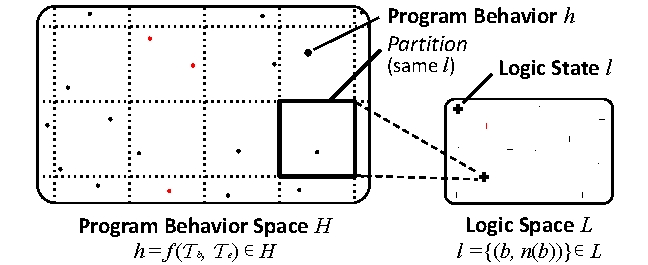
\includegraphics[width=\columnwidth]{images/prog-to-logic.pdf}
  \caption{The program behavior space and the logic space. Red indicates
  abnormal program behaviors or logic states}.
  \label{f:prog-to-logic}
\end{figure}

\pp{Logic state and logic space}
%
A \emph{logic state} $l$ is a set of all satisfied branches during execution,
which is essentially the order-ignored version of a branch history. Formally,
given a branch history $\mathcal{T}_b$ of an execution,
%
\begin{equation}
\label{e:ls}
  l := \{b \mid b \in \mathcal{T}_b\}.
\end{equation}

A \emph{logic space} $\mathbb{L}$, then, is a set of all possible logic states
of a given program. 
%
It is possible to see a logic space as the \emph{subdivision} of a program
behavior space along logic states. \autoref{f:prog-to-logic} shows the
relationship between a program behavior space and a logic space, where each
\emph{partition} of a subdivided program behavior space corresponds to one logic
state. 


\pp{Logic state coverage}
%
\emph{Logic state coverage} is \emph{the count of observed distinctive logic
states during fuzzing}, where a logic state is called \emph{covered} when
fuzzing observed a program behavior that belongs to such a logic state (i.e.,
triggering all and only the branches in the logic state). 
%
Analogically, logic state coverage represents the \emph{covered area} of a logic
space.

Logic state coverage is crucially distinguished from edge coverage in that, 
while edge coverage merges all observed edge traces into one, logic state
coverage distinguishes every logic state and counts them individually. This
enables logic state coverage to count underlying program behaviors independent 
of what has been observed before, while edge coverage unpredictably ignores some
of them as it is heavily affected by the previous observation.

As shown in \autoref{f:prog-to-logic}, a logic state (i.e., a partition in the
program behavior space) may contain various program behaviors, suggesting a
single covered logic state may encompass several different behaviors. However,
in \autoref{s:prop}, we explain that a logic state is representative of
interesting program behaviors as it (i) reflects the interestingness of
underlying program behaviors and (ii) only contains the program behaviors of the
same normality.


\section{Representativeness of Logic States}
\label{s:prop}

In this section, we discuss the desirable properties of logic states to
represent interesting program behaviors (\autoref{s:prop:prop}). Then, we
continue to discuss how logic states have such properties
(\autoref{s:prop:repr} and \ref{s:prop:local}).

\subsection{Desirable Properties}% as a Proxy Metric}
\label{s:prop:prop}

\pp{Interestingness}
%
Logic states should be sufficiently representative of the \emph{interesting}
program behaviors. Specifically, it should distinguish most program behaviors
deemed interesting while not over-representing less interesting ones. 

\pp{Normality}
%
The \emph{normality} of all program behaviors should be uniform (i.e., the same)
within a logic state. Otherwise, the normality of one observed program behavior
cannot represent that of other behaviors in the same logic state.
%
%\pp{Feasibility}
%%
%Measuring logic state coverage should be \emph{feasible} to implement. In other
%words, the measurement mechanism should be clear and the implementation
%requirement should not be unrealistic. 

\begin{figure}[t]
  \centering
  \vspace{-1em}
  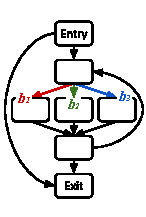
\includegraphics[height=4.5cm]{images/repr-cfg.pdf}
  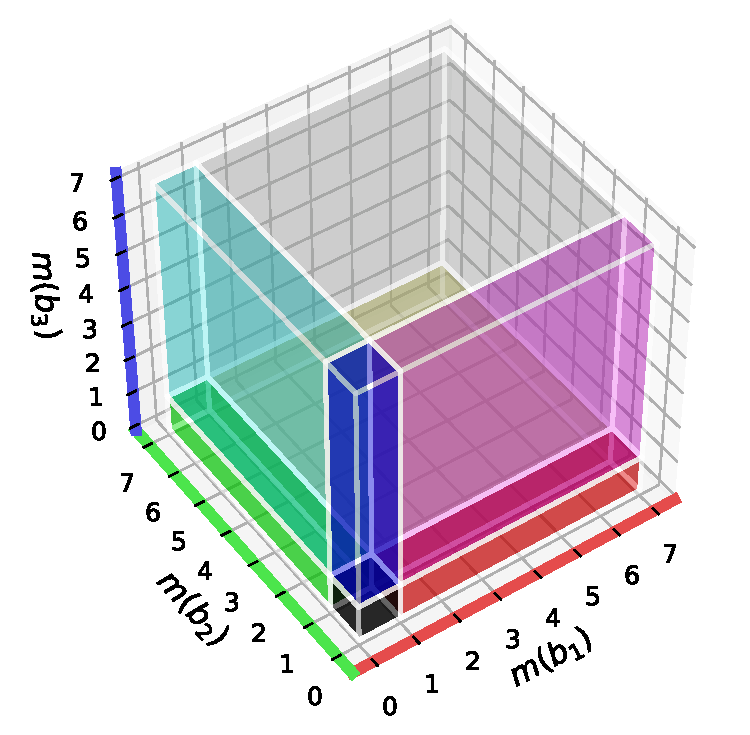
\includegraphics[height=4.5cm]{images/repr-grid.pdf}
  \vspace{-.5em}
  \caption{Example control flow graph and its logic states (colored box) that
  the program behaviors with different branch hit counts belong to. $m(b)$
  denotes the hit count of branch $b$.}
  % Each region surrounded by dotted lines constitutes one logic state.}
  \label{f:repr}
\end{figure}

\subsection{Interestingness}
\label{s:prop:repr}

Logic states coalesce less interesting program behaviors that exhibit more
branch repetitions in a fewer logic states, resulting in smaller (larger) logic
state coverage as it observes more uninteresting (interesting) program
behaviors.

%This is because logic
%states lump together larger hit counts into fewer integer buckets
%(\autoref{e:ls}).

\autoref{f:repr} shows an example control-flow graph and its logic space,
gridded up by the different hit counts $m(b)$ of the branch $b_1$, $b_2$, and $b_3$.
%, where $m(b)$ denotes the hit count of a branch $b$. 
Each colored box represents one logic state, which includes all program
behaviors that fall into the box.
For example, a program behavior that does not hit any of $b_1$, $b_2$, and $b_3$ 
(i.e., $m(b_1)=m(b_2)=m(b_3)=0$) belongs to the \cbox{black} logic state, while
all program behaviors that hit only $b_1$ (i.e., $m(b_1)>1$ and
$m(b_2)=m(b_3)=0$) fall into \cbox{red}.
%, and all program behaviors that hit only $b_2$ and $b_3$ (i.e.,
%$m(b_1)>1$, $m(b_2)>1$, and $m(b_3)=0$) fall into the \cbox{cyan} logic state.

The colored boxes in \autoref{f:repr} suggest the increasing size of logic
states as their constituent program behaviors involve more repetitive branches.
To be specific, a logic state covers a progressively larger volume 
in the logic space 
(i.e., \cbox{black} $\rightarrow$ \cbox{red}/\cbox{green}/\cbox{blue}
$\rightarrow$ \cbox{yellow}/\cbox{cyan}/\cbox{magenta} $\rightarrow$
\cbox{gray}) as it contains more repetitive branches (i.e., 0 $\rightarrow$ 1
$\rightarrow$ 2 $\rightarrow$ 3 repetitive branches). 
%
This results in repetitive (i.e., uninteresting) program states packed
to fewer logic states, suppressing (boosting) logic state coverage as it observes more
uninteresting (interesting) behaviors.
%\footnote{It is worth noting that a coordinate in the grid does
%\emph{not} represent one program behavior. For example, a coordinate (1, 1, 0)
%represents two program behaviors, $b_1$ before $b_2$ and $b_2$ before $b_1$.
%However, it does not affect the relative size of visualized logic states because
%a coordinate only has more program behaviors as it gets further from the
%origin.}

%%Notice that a program behavior is deemed more interesting as it exhibits
%%smaller branch hit counts (\autoref{s:fuzz:unfuzz}). 
%As shown, a logic state distinguishes more interesting program behaviors in a
%finer granularity, representing fewer behaviors with smaller branch hit counts
%(i.e., bottom left). On the other hand, it coalesces more behaviors when
%the branch hit counts get larger, where individual behaviors are deemed less
%interesting. 
%%
%This results in a larger number of covered logic states when the observed
%behaviors are more interesting (e.g., three program behaviors result in
%three different logic states when $m(b_3)<2$) while the opposite happens when
%they are not (e.g., a total of 11,950 behaviors fall into \emph{one} logic state
%when $4 \le m(b_1) < 8$ and $4 \le m(b_2) < 8$).

\begin{figure}[t]
  \centering
  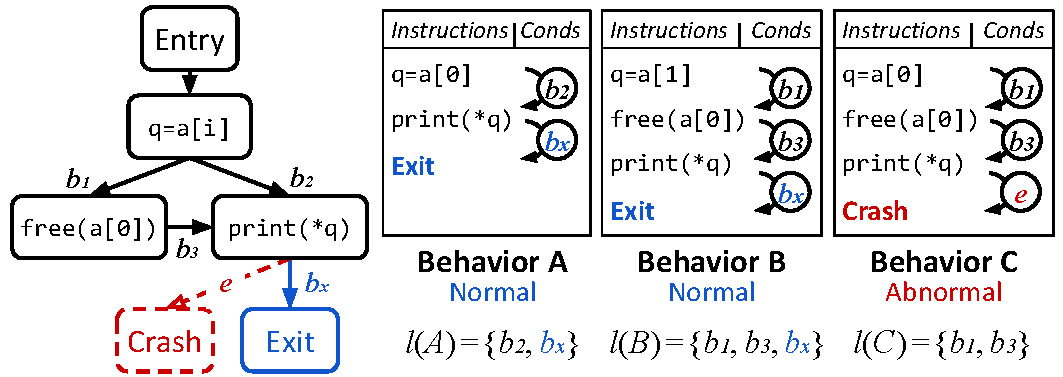
\includegraphics[width=\columnwidth]{images/local.pdf}
  \caption{Example control flow graph and program behaviors. The exceptional
  condition $e$ is satisfied when the memory pointed by $q$ is a freed
  memory. $l(X)$ denotes the logic state of a program behavior $X$.}
  % Each region surrounded by dotted lines constitutes one logic state.}
  \label{f:local}
\end{figure}

\subsection{Normality}
\label{s:prop:local}

Given that a program does not exhibit an exception exactly at the program exit
point, all program behaviors in one logic state have the same normality, namely
either normal or abnormal altogether.
%
This is because normal behaviors trigger the \emph{exit branches} that
lead to the exit point, while abnormal behaviors do not. Since the logic
states of two behaviors are always distinguished by exit branches, they cannot
have the same set of satisfied branches (i.e., the same logic state).

\autoref{f:local} shows an example program that contains a use-after-free
exception $e$, which is satisfied when the memory pointed by $q$ belongs to
freed memories. Three example program behaviors and their logic states are shown
on the side. Since normal behaviors (Behaviors A and B) terminate at the program
exit, their logic states contain the exit branch $b_x$ that directly leads to
the program exit. On the other hand, since the abnormal behavior (Behavior C)
triggers the exception $e$ that crashes the execution before reaching the
program exit, its logic state does not contain any exit branch unlike normal
behaviors.

%
%\subsection{Feasibility of Measurement}
%\label{s:prop:feasi}
%
%% concerns: space and time.
%%  - time: less important, unless the overheads are too prohibitive for real-time usage.
%%    - reason: this measurement is only for evaluation, not for practical use.
%%  - space: main concern, because a program behavior space is presumably large (i.e., a
%%    huge number of program behaviors expected). shouldn't be unrealistic.
%% step-by-step procedure
%%  1. record the logic state of an execution
%%  2. add it to the observed set
%%  3. count the number of elements in the set
%% feasibility of steps
%%  1. (space) exactly the same as the overheads of coverage instrumentation.
%%  2. (space) rough upper bound of the number of logic states is manageable.
%%     - set implementations proportional to the number of elements.
%%  3. (space) wouldn't require more non-trivial space (compared to the set itself).
%
%% TODO: "unrealistic?"
%
%Measuring logic state coverage has a clearly defined procedure to follow, which 
%does not require any unrealistic implementation. Two main concerns regarding 
%implementation are \emph{temporal} and \emph{memory} overheads, but we note
%that temporal overheads are relatively unimportant as the purpose of the
%measurement is \emph{evaluation} (i.e., comparing fuzzers), not for the actual
%fuzzing campaign. Memory overheads, on the other hands, are the actual concern
%as the size of a logic space is expected to be huge (i.e., massive number of
%possible logic states). However, we show that the memory requirement is also not
%prohibitive in the following.
%
%\pp{Step-by-step procedure}
%%

\section{Measuring Logic State Coverage}
\label{s:measure}

In this section, we first summarize the high-level procedure of logic space
coverage measurement and its subsequent requirements 
%to ensure fairness across different fuzzers 
(\autoref{s:measure:req}). Then, we introduce a \emph{bloom filter} as an
effective way to achieve the requirements (\autoref{s:measure:bloom}).


\subsection{High-level Procedure}
\label{s:measure:req}

% - minimal computation overhead 
% - constant computation overhead 
% - feasible memory overhead

%\pp{Procedure}
%
%At a high level, measuring logic state coverage can be described with the
%following procedure:
At a high level, the measurement can be described as follows:

\begin{enumerate}[noitemsep,label=\arabic*)]
  \item \emph{Record} a logic state per execution.
  \item \emph{Add} the logic state to a set of observed logic states.
  \item \emph{Count} the size of the set, yielding logic state coverage.
\end{enumerate}

In this procedure, recording a logic state (1) is technically identical to edge
tracing in coverage-guided fuzzers \cite{afl,fioraldi2020aflpp,libfuzzer}.
Managing logic state coverage (2 and 3), on the other hand, poses an extra
challenge as fuzzers are expected to observe a myriad of distinct logic states
during a campaign.


\pp{Requirements}
%
As the purpose of logic state coverage is comparing (i.e., evaluating) different
fuzzers, the measurement should not induce any bias to certain fuzzers. To this
end, it should satisfy the following requirements.

\begin{itemize}
%  \item \textbf{R0. Measurement accuracy.}
%    The measurement should yield a reliable number that properly captures logic
%    state coverage without a significant error.

  \item \textbf{R1. Light computation overheads.}
    %Although the coverage measurement is only for evaluation, 
    The computation overheads should not be heavy. Otherwise, it would overshadow
    the benefit of fast fuzzing executions, penalizing high-speed fuzzer designs
    \cite{sergej2021nyx,schumilo2020hypercube,song2020agamotto}.
    % NOTE: "heavy" not well defined.

  \item \textbf{R2. Constant computation overheads.}
    The measurement overheads should not increase as logic state coverage
    expands. Otherwise, it would penalize the fuzzers with larger logic space
    coverage.

  \item \textbf{R3. Feasible memory overheads.}
    The memory requirement for the measurement should be feasible for commodity
    evaluation settings for practical reasons.
    % NOTE: "feasible" not well defined.
\end{itemize}


\subsection{Leveraging a Bloom Filter}
\label{s:measure:bloom}

\begin{figure}[t]
  \centering
  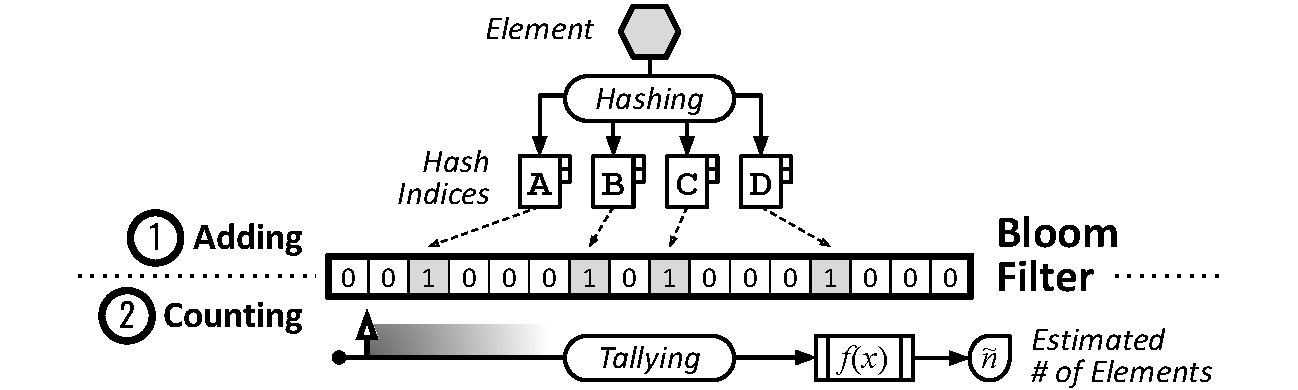
\includegraphics[width=\columnwidth]{images/bloom.pdf}
  \caption{Operation illustration of a bloom filter.}
  \label{f:bloom}
\end{figure}

% why bloom filter
% introduction

For logic state coverage management, we employ a \emph{bloom filter} that 
offers an %computationally and spatially 
efficient set implementation at the cost of manageable inaccuracy (i.e., false
positives).
%
%\pp{Operation summary}
%
\autoref{f:bloom} illustrates the basic operations of a bloom filter. Starting
from an array of 0s, it \emph{adds} an element by setting the hash indices to 1
and \emph{counts} the number of elements by tallying 1s in the filter and
applying it to the counting formula (\autoref{e:count}).


% usage: logic state (element), a set of observed logic states (filter)
% tight error bounds, which can further be suppressed by parameters (R0)
% hash and formula calculation (R1)
% constant-time adding / counting (R2)
% irrelevant to the actual size of an element (R3)
%
\pp{Usage and benefit}
%
In the measurement, a bloom filter represents \emph{a set of observed logic
states}, which accepts a logic state every execution and yields logic state
coverage via the number of elements in the set. It only requires a few
computations for hashes and the counting formula (\textbf{R1}), both of which
are nearly $O(1)$ as the number of hashes and the filter size are fixed
(\textbf{R2}). Furthermore, the filter size is entirely agnostic to the size of
a logic state thanks to hashing (\textbf{R3}). 

\pp{Deciding parameters}
%
A bloom filter may introduce some inaccuracy by construction. However, it can
be reliably suppressed by the choice of data structure parameters, namely the
filter size (i.e., the number of bits) $n_b$ and the number of hashes $n_h$.
They can be optimally determined by the maximum expected number of elements
$n_e$ and the desired false positive probability $\epsilon$ by the following
equations \cite{tarkoma2012bloom}:
%
\begin{equation}
  n_b = -n_e\ln{\epsilon}/(\ln{2})^2, \enspace n_h = -\log_2{\epsilon},
  \label{e:param}
\end{equation}

In our setting, $n_e$ corresponds to the upper bound of \emph{observable
distinct logic states} during a fuzzing campaign. To conservatively estimate
$n_e$, we adopt three premises in ideal evaluation : (i) fuzzing continues for
the maximum 24 hours, (ii) a fuzzer executes the maximum 1,000 inputs per
second, and (iii) \emph{every} execution yields a distinctive logic state. Then, 
%
\begin{align}
  n_e &= \SI{24}{\hour} \times \SI[per-mode=symbol]{3600}{\second\per\hour}
         \times \SI[per-mode=symbol]{1000}{\exec\per\second} 
         \times \SI[per-mode=symbol]{1}{\state\per\exec} \nonumber \\
      &= \SI{86.4e+6}{\state} 
         \approx \SI[parse-numbers=false]{84 \times 2^{20}}{\state}. \nonumber
\end{align}

Assigning the upper bound $n_e$ and a reasonable false positive probability
$\epsilon=0.05$ to \autoref{e:param} yields:
%
\begin{equation}
  n_b = \SI{538e+6}{\bit}\approx\,\SI{512}{\mbit}=\SI{64}{\mb}, \enspace n_h = 4.32 \approx 4. \nonumber
\end{equation}

Notice that adding a logic state only requires calculating four hashes per
execution (\textbf{R1} and \textbf{R2}) and the memory overhead ($\SI{64}{\mb})$
is also marginal to a commodity setup (\textbf{R3}). 


\pp{Counting elements}
%
Along with data structure parameters, a counting formula that estimates the
number of elements may also affect the accuracy of logic state coverage.
Papapetrou et al. \cite{papapetrou2010cardinality} proposed a high-accuracy
counting formula that calculates the estimated number of elements
$\tilde{n}_e(X)$ when the number of 1s in the filter is $X$ as follows:
%
\begin{equation}
  \tilde{n}_e(X) = \frac{\ln{(1-X/n_b)}}{n_h \ln{(1-1/n_b)}}.
  \label{e:count}
\end{equation}

\autoref{e:count} comes with three major benefits. First, it offers one of the
best accuracy among all alternatives (c.f., only 4\% error even in an extreme
filter density of 90\%)
\cite{harmouch2017cardinality,papapetrou2010cardinality}. 
%, while its error rate is \emph{inversely proportional} to the actual number of
%elements in the set (i.e., even \emph{less} error as logic state coverage
%grows) \cite{harmouch2017cardinality}. 
%
Second, it allows for a near-constant-time calculation as it only requires the
number of 1s apart from the formula calculation, as well as empirically shown in
\cite{harmouch2017cardinality} (\textbf{R2}). 
%
Finally, it presents a calculable error bound that the actual number of elements
likely falls within given a confidence probability \cite{papapetrou2010cardinality}.

% TODO: fast logarithm calculation? or empirical?
% TODO: error bound formula.


\section{Design and Implementation}
\label{s:design}

%To satisfy the requirements, we incorporate a \emph{bloom filter} to manage a
%set of observed logic states. 
In this section, we first present the design overview (\autoref{s:design:over})
and elaborate on details (\autoref{s:design:rec} and \ref{s:design:count}).


\begin{figure}[t]
  \centering
  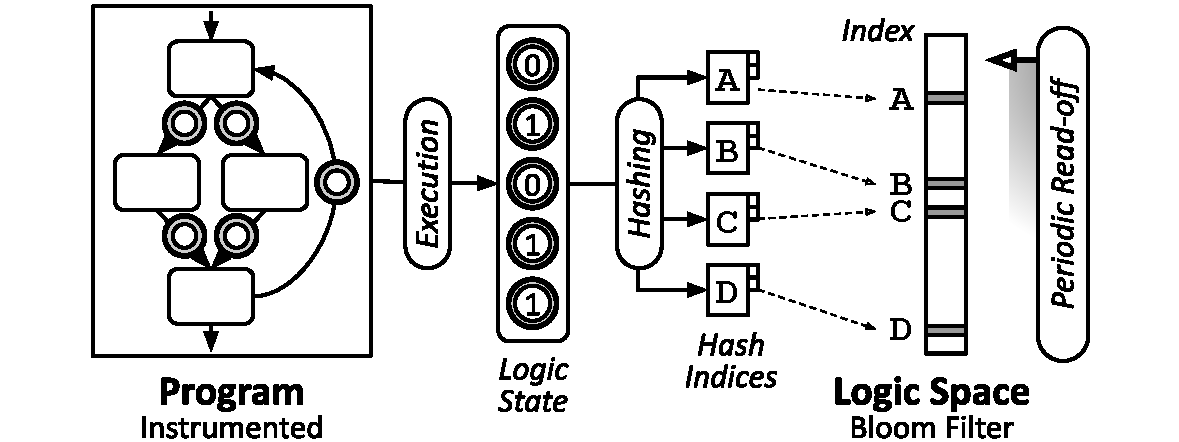
\includegraphics[width=\columnwidth]{images/design.pdf}
  \caption{Logic state coverage measurement overview.}
  \label{f:design}
\end{figure}


\subsection{Overview}
\label{s:design:over}

% basics: record distinct logic states to a bloom filter, and estimate # later.
%  - (1) for each execution, edge trace -> N hash(edge trace)'s
%  - (2) insert N hash(edge trace)'s to the bloom filter.
%  - (3) periodically estimate the # of distinct edge traces = logic states.

\autoref{f:design} illustrates the workflow of logic state coverage
measurement. Similar to edge coverage, it first records the \emph{logic state}
of each execution via instrumentation (\autoref{s:design:rec}). Then, it adds
the recorded logic state to a \emph{bloom filter} that represents a set of
observed logic states, by setting the hash indices (\autoref{s:design:up}).
Finally, the measurement periodically reads off the bloom filter to count the
number of observed logic states (\autoref{s:design:count}).


\subsection{Recording a Logic State}
\label{s:design:rec}

% summary: similar to the conventional edge tracing in coverage-guided fuzzing.
%  - create a edge hash combining two consecutive basic block hashes.
%  - increase the hit count of each each hash whenever it visits it.
%  - bucket the hit counts into their integer logarithms.
% meaning
%  - edge hash --> branch in a logic state
%  - bucketed hit count --> bucket of the corresponding branch
%  - entire bucketed edge trace --> logic state
% overheads
%  - (R1) proven by practice.
%  - (R3) minimal memory requirement -- around 64KB.


\subsection{Updating Logic State Coverage}
\label{s:design:up}

% intro: bloom filter
% summary
%  - create hashes of a logic space.
%  - set the indices of the bloom filter, indicated by the hashes.
% determining bloom filter parameters
%  -


\subsection{Counting Logic State Coverage}
\label{s:design:count}



\section{Experiment}

\subsection{Experiment Setup}

\subsection{Measurement Overheads}

\subsection{General-purpose Fuzzing}

\subsection{Hypervisor Fuzzing}

% same cov: what can we learn more from logic state cov?

\subsection{Grammar Fuzzing}

% init corpus cov: what can we learn more from logic state cov?


\section{Discussion}
\label{s:disc}

\pp{Completeness of untargeted fuzzing}
%
Unlike comparative quality that only requires to compare the number of observed
distinct program behaviors, it is difficult to measure the absolute
\emph{completeness} of untargeted fuzzing that requires to measure how much a
program has been completely verified. This is because the total number of
program behaviors is unknown: if it can be known, then we would already know
which abnormal behaviors are possible, precluding the necessity of fuzzing in
the first place.

One possible compromise is performing preliminary static analysis to
\emph{estimate} the total number of program behaviors, including abnormal ones.
However, it would pose a potential problem that the estimated 100\% completeness
does not necessarily mean the actual 100\% completeness, which may compromise
the very purpose of measuring absolute completeness.

\pp{Generalization to multi-thread programs}
%
Unlike single-thread programs, \emph{multi-thread} programs may concurrently
execute multiple basic blocks. In this case, a program behavior (i.e., a stream
of executed instructions) also depends on the thread interleaving in
addition to the branch and exception histories, which breaks the proxy
properties of a logic space (i.e., interestingness and normality).
An alternative proxy of comparative quality may be proposed by either
extending logic state coverage or devising yet another coverage metric.

\pp{Normality of a partial logic state}
%
It is crucial to notice that an abnormal behavior \emph{still follows the
regular control flow up until any exception happens}. In \autoref{f:local}, the
abnormal behavior (Behavior C) follows the same control flow to a normal
behavior (Behavior B) until use-after-free, which makes the behavior eventually
abnormal unlike its normal counterpart. 
%
What it implies is that the executions that do not contribute to the growth of
logic state coverage are not entirely wasteful executions because they are still
possible to reveal abnormal behaviors. However, they are unlikely to do so, let
alone revealing \emph{unknown} ones (\autoref{s:fuzz:unfuzz}).

%This means that, even though a behavior is known to be normal, it does not
%suggest much about the normality of other behaviors \emph{on course for} such.

%At a high level, this can manifest when multiple inputs trigger the same
%branches but only some of them satisfy exceptions (e.g., due to different data
%values).

%\pp{Interestingness: definition vs. convention}
%%
%Although the \emph{interestingness} has been widely discussed in recent
%untargeted fuzzing, it has never been clearly defined. The conventional
%understanding is a property of an \emph{input} having \emph{new
%execution paths} in its resulting behavior. In comparison, this work
%defines interestingness as a property of a \emph{program behavior} indicating 
%the \emph{expectation} of being an abnormal behavior. 
%
%Despite an apparent difference between them, the definition \emph{subsumes} the
%convention because if an input discovered a new path (conventional
%interesting), its behavior would have a higher expectation to be abnormal than
%the ones only exhibiting previously checked paths (defined interesting). 
%%
%Still, there are some disagreements between the definition and the convention,
%such as when a behavior \emph{contains} another known abnormal behavior without
%discovering any new path. The definition may be refined to resolve such
%disagreements.

%\pp{Completeness of targeted fuzzing}
%%
%The completeness of untargeted fuzzing hinges on the observation that the more
%interesting program behavior it checks, the less unknown abnormal program
%behaviors are expected to be left. This roughly translates to $\Pr(\mathrm{UA}
%\mid \mathrm{N})$ being equal throughout a fuzzing campaign.
%%, whereby $\Pr(\mathrm{new} \cap
%%\mathrm{abnormal})$ then majorly depends on how high $\Pr(\mathrm{new})$ is;
%%proportional to the number of observed program behaviors per time.
%%
%However, targeted fuzzing (e.g., directed or regression fuzzing)
%\emph{prioritizes} code that likely leads to abnormal behaviors, which may result
%in a larger $\Pr(\mathrm{UA} \mid \mathrm{N})$ at the beginning that slowly
%decreases over time. 
%
%This affects the fundamental observation for completeness because targeted
%fuzzers may reveal more abnormal behaviors even after observing fewer program
%behaviors.
%%
%One possible remedy is refining interestingness to incorporate a complete set of
%factors that affects $\Pr(\mathrm{UA})$ (e.g., freshness of code).  A
%further investigation on interestingness is required.

% FIXME: revise!
\pp{Quality metric for general fuzzing}
%
Logic state coverage evaluates the quality of \emph{untargeted} fuzzing, where
the program behaviors with less repetition are generally deemed more
interesting. 
%
However, \emph{targeted} fuzzing
\cite{aflchurn,chen2020savior,osterlund2020parmesan,lee2024syzrisk} attempts to
capitalize the recent findings \cite{aflchurn,zhai2022ndss,nikolaos2022longvuln}
that some code such as recent patches are potentially \emph{more interesting}
(i.e., likelier to cause abnormal behaviors), which may render logic state
coverage to under-estimate targeted fuzzing by overlooking potentially
interesting behaviors.

To devise a quality metric that also encompasses targeted fuzing, future
research may need to address two issues revolving around interestingness. First,
it should accurately describe the interestingness in an impartial way (i.e., not
favoring a certain fuzzer or setting). To do so, it should assess which factor
affects interestingness and how much more than one another. Second, it should
incorporate such a description into the quality metric. Should it follow the
philosophy of logic state coverage, grouping uninteresting behaviors may be a
possible approach to make them less significant.


\pp{Alternative ways to manage logic state coverage}
%
There has been much research work regarding how to estimate the cardinality
(i.e., the number of elements) in a set in an efficient way
\cite{papapetrou2010cardinality,harmouch2017cardinality}, where using a bloom
filter is just one of the approaches. Harmouch et al.
\cite{harmouch2017cardinality} evaluated different cardinality approximation
approaches and compared their accuracy with various benchmarks.  Although using
a bloom filter is the most recent approach compared in the paper, other
alternative approaches can be incorporated to manage logic state coverage as it
is not always the optimum solution.


\pp{Semantically abnormal behaviors}
%
While the definition of program behaviors is separated from the output, it can
still incorporates \emph{semantically} abnormal behaviors (i.e., semantic bugs)
by means of exceptions. To be specific, semantic error detection such as
semantic sanitizers \cite{kim2019hydra,yun2016apisan} may capture semantic bugs
on the fly and make the behavior abnormal by terminating it. The definition
allows this because the output is just an observable subset of the data context
during the execution, which exceptions can reference at runtime.


\section{Related Work}

\pp{Reliability of conventional metrics}
%
Since the advent of popular fuzzing, researchers have consistently
called into question a method to evaluate fuzzers. Klees et al.
\cite{klees2018evaluating} evaluated then state-of-the-art fuzzers and raised an
issue about using edge coverage and the number of discovered bugs as quality
metrics. \textsc{UniFuzz} \cite{li2021unifuzz} also pointed out that such
metrics are incomprehensible and lead to incomplete assessment. B\"{o}hme et al.
\cite{bohme2022reliability} also noted that edge coverage does not strongly
represent the comparative quality between fuzzers.  While they all suggest the
necessity of an alternative quality metric, it has yet to be proposed and widely
accepted in practice. 

\pp{Alternative metrics}
%
Some researchers did propose alternative metrics for coverage-guided fuzzing
\cite{wang2020notallcov,wang2019impactcov,yan2020pathafl,gan2020greyone,gan2018collafl}.
However, they are commonly meant for \emph{performance} (e.g., more bugs or edge
coverage), not for \emph{comparison}, which makes using such metrics for
comparison likely yield an unjustified advantage toward certain fuzzers.
%
\textsc{Sand} \cite{kong2024sand} proposed \emph{execution patterns}
(conceptually similar to logic states) to enable fuzzing without sanitization.
However, similar to other alternative metrics, it was never meant for
comparative evaluation nor correlated to the fuzzing quality. 
%designed for them.

\pp{Evaluation methods and platforms}
%
%Similar to the relative completeness argument (\autoref{s:fuzz:unfuzz}),
B\"{o}hme et al. \cite{bohme2021residual} proposed a technique to estimate the
probability of discovering more bugs,
%using its edge coverage trend.  However, the expected maximum number of bugs
%highly depends on the capability of individual fuzzers, which makes it
%impossible to directly compare the estimated probabilities between fuzzers.
but the probability cannot be directly compared between fuzzers as it highly
depends on the capability of individual fuzzers.
% to each other.
%
\textsc{UniFuzz} \cite{li2021unifuzz} and \textsc{FuzzBench}
\cite{metzman2021fuzzbench} presents a platform to comparatively evaluate
fuzzers in multiple metrics. 
%including edge coverage and the number of bugs, 
%While the use of multiple metrics is susceptible to an interpretation bias,
%and does not provide a reliable agreed-upon quality measure.
%
Logic state coverage can be readily incorporated into the platform as a quality
metric.



\section{Conclusion}


%-------------------------------------------------------------------------------
% BIBLIOGRAPHY
%-------------------------------------------------------------------------------

% NOTE: Commented out just until I make the first citation.
\bibliographystyle{plain}
\bibliography{main}

%-------------------------------------------------------------------------------
% APPENDIX
%-------------------------------------------------------------------------------

\begin{appendix}

\end{appendix}

\end{document}
